% Created 2022-12-01 יום ה 10:47
% Intended LaTeX compiler: pdflatex
\documentclass[11pt]{article}
\usepackage[utf8]{inputenc}
\usepackage[T1]{fontenc}
\usepackage{graphicx}
\usepackage{longtable}
\usepackage{wrapfig}
\usepackage{rotating}
\usepackage[normalem]{ulem}
\usepackage{amsmath}
\usepackage{amssymb}
\usepackage{capt-of}
\usepackage{hyperref}
\author{Jonathan Sahar}
\date{\today}
\title{How to analyze fMRI}
\hypersetup{
 pdfauthor={Jonathan Sahar},
 pdftitle={How to analyze fMRI},
 pdfkeywords={},
 pdfsubject={},
 pdfcreator={Emacs 28.1 (Org mode 9.5)}, 
 pdflang={English}}
\usepackage{biblatex}

\begin{document}

\maketitle


\section{connect to the MRI center file}
\label{sec:org5b743e0}
\subsubsection{Other locations in file manager}
\label{sec:org123b17a}
\subsubsection{smb://mrilabfs.tau.ac.il/mri\textsubscript{XX}\textsubscript{lab}\$}
\label{sec:orge88f15b}
\subsubsection{username/password - same as in TAU}
\label{sec:org10ac99a}


\section{Order the data on my computer:}
\label{sec:org6e781f0}
\subsection{BIDS  folder structure}
\label{sec:orga595d4e}
The standard way to order and share imaging data
\url{https://bids.neuroimaging.io/}

Batel has a script for that :)

\section{types of scans}
\label{sec:org5ceac9a}
\subsubsection{Mprage - anatomical}
\label{sec:org633bc34}
\subsubsection{cmrr - functional}
\label{sec:org18adb09}
\subsubsection{each scan name contains the number of volumes, and a name we can choose}
\label{sec:org634b438}
\subsubsection{there's an \_sbref scan for each scan: used for motion correction, we don't use it usually}
\label{sec:org7aeff1b}
\subsubsection{each dicom is 3D at a given Tr}
\label{sec:org4f25fd2}
\subsubsection{use the 2nd mprage dir - has been filtered}
\label{sec:orgf2a01a7}
\section{analyzing with FSL}
\label{sec:org312cf0d}
Can open individual tools from command line - for GUI, call tool with capital letter (otherwise is calls the function directly)
\subsection{BET}
\label{sec:org8d8647a}
Extract the brain only
need to do only once - for the anatomical data, FEAT later uses it
give it the anatomical DICOM

\subsection{FEAT - first level}
\label{sec:orge4651f4}
\subsubsection{Data:}
\label{sec:orge280e07}
Preprocessing \& GLM analysis
first level: single run
second level: multiple runs
group analysis
fulle analyis = inc. running a GLM
highpass filter = 100HZ

\subsubsection{pre-stats}
\label{sec:org8f5a8a6}
Keep defaults, and add slice time correction = interleaved

\subsubsection{registration}
\label{sec:orgd9293ff}
Select anatomical\textsubscript{brain} image (from BET)
for the standard space use full search \& 12 DOF

\subsubsection{Stats}
\label{sec:orgd2f318b}
Need to create an EVs (events) files for every kind of event that happend in the scan:
\begin{center}
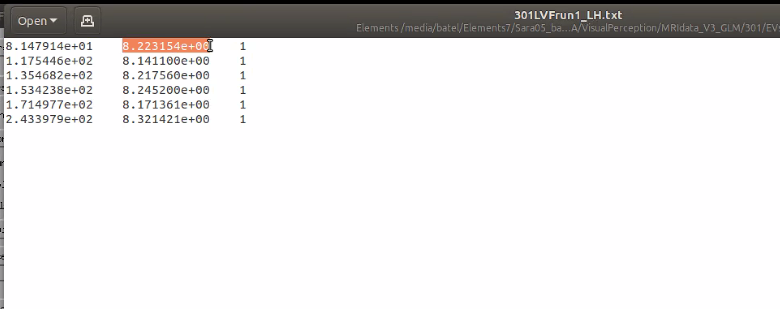
\includegraphics[width=.9\linewidth]{c:/mnt/g/My Drive/notes/slip-box/2022-04-27-121446-how_to_analyze_fmri.org_20220427_130611_bCeBCg.png}
\end{center}
onset  duration weight

The GLM: ``Full model  setup''
create a page for each EV
HRF: double gamma

\subsubsection{post-stats = multi comparisons correction}
\label{sec:org3c655bc}
Don't need for first-

\subsubsection{save!  before hitting go}
\label{sec:org7ea1f8d}
Creates a ``batch'' file : .fsf

\subsubsection{go}
\label{sec:org6d3df76}
Creates a FEAT report html that updates in real time
shows the quailty of registration, motion correction, the details of the statistical model etc.

Can run from command line as ``feat path/to/design.fsf''

\subsubsection{load}
\label{sec:orgb4c42ba}
load an existing .fsf file
can create an empty .fsf with names of vars in ``'', and then populate file with a script


\subsubsection{output:}
\label{sec:orgb194ba1}
Work with filtered\textsubscript{Func}\textsubscript{data} feed into FSLeye

cope files: the different contrasts we computed: we can use them later for the higher order analysis.

in stat directory:
\begin{itemize}
\item peNUM: the beta value for each eventNUM in EVs: also NIFTI files, the beta for each voxel
\item tfiles - the t-values for each voxel
\end{itemize}

Feat doen't apply the transformation to MNI - the coomputations for doing so are in reg dir.
Also in reg - hires\textsubscript{head} - the anatomical head

\subsection{FEAT - higher level}
\label{sec:orgf346807}
Analyze multiple runs from the same esubject
input the cope files from previous analysis of all runs
averages the different run + transforms to MNI space

\subsection{FSLeyes}
\label{sec:orga33e4ba}
Presentation of images

\subsection{dcm2nii - external app}
\label{sec:org9cffe3b}
Convert DICOM to NIFTI

\section{more info on FSL - videos from jeanette mamford \url{https://www.youtube.com/watch?v=lCwewJJPd5U\&list=PLB2iAtgpI4YHlH4sno3i3CUjCofI38a-3}}
\label{sec:org40ecc9a}
\section{Code -}
\label{sec:orge30e7c9}
main\textsubscript{visualPerceptionAnalysis.m} in Batel's code base
\end{document}
